\documentclass{cygclanek}
\addbibresource{example_ref.bib}
\begin{document}

\title{Návod k šabloně}

\names{
    \name[*]{Matěj Rzehulka}{fjfi}, \name{Jára Cimrman}{nerc,abc}, \name{Bilbo Baggins}{fvu,nerc}, \name{Frodo Baggins}{nerc}
}
\institutions{
    \institution{fvu}{Fiktivní výzkumný ústav, Neexistující ulice 5, 999 99 Nikde, ČR}
    \institution{nerc}{Non-existing research centre, 5.25 New street, SM PSTCD, Some Country}
    \institution{abc}{Somewhere}
    \institution{fjfi}{FJFI ČVUT v Praze, Břehová 7, 115 19 Praha 1, ČR}
}

\email{rzehumat@fjfi.cvut.cz}
\year{2022}

\maketitle
\begin{abstract}
    Abstrakt napište mezi \verb|\begin{abstract}| a \verb|\end{abstract}|.
\end{abstract}
\keywords{Klíčová slova napište do tagu keywords.}

\section{Úvod}

Tento dokument slouží jako návod. 

\section{Teorie}
Tady demonstrujeme několik možností, jak tuto šablonu používat.

\subsection{Izotopy, reakce, chemie}
Izotopy lze psát pomocí \verb|\ce|, např. \verb|\ce{^{2}D}| vytvoří \ce{^{2}D}. Podobně to lze použít i na 
reakce - např. \verb|\ce{^{10}B(n,\alpha) ^7Li}| je \ce{^{10}B(n,\alpha) ^7Li}. Alternativně lze 
použít i šipku, což se dá napsat jako\newline\verb|\ce{^{10}B + n -> ^4He + ^7Li}| 
a vytvoří \ce{^{10}B + n -> ^4He + ^7Li}. 

Pomocí \verb|\ce| lze psát i chemické reakce, např.\verb|\ce{H2SO4 + 2NaOH -> Na2SO4 + 2H2O}| vytvoří \ce{H2SO4 + 2NaOH -> Na2SO4 + 2H2O}.

    Prostředí \verb|\ce| je \uv{univerzální}, lze jej používat jak v textu, tak i v matematickém módu 
    (tj. části vymezené \verb|{$...$}|, \verb|$$ ... $$|, \verb|\begin{equation}...\end{equation}| atd.

Prostředí \verb|\ce| pochází z balíčku \verb|mhchem| \cite{ctan_mhchem} (není třeba nic přidávat 
pomocí \verb|\usepackage|, balíček už je zahrnut v~\verb|documentclass|).

\subsection{Čísla, jednotky}
Čísla se mohou normálně psát do textu, jako 2, 3, 314,579 atd. To však má několik 
problémů - mezera mezi tisícemi se nedělá automaticky, desetinnou tečku/čárku nelze hromadně měnit, 
zápis nejistot je velmi pracný, atd.

Lepší je používat příkaz \verb|\num| z balíčku \verb|siunitx| \cite{ctan_siunitx} (už přidáno 
v rámci šablony). Např. \verb|\num{5672684}|, \verb|\num{3.25e6}|, \verb|\num{2.25(1)e6}| vytvoří 
\num{5672684}, \num{3.25e6}, \num{2.25(1)e6}. Pro dlouhý zápis chyby pak lze použít 
\verb|\num[separate-uncertainty=true]{2.25(1)e6}|, což vytvoří \num[separate-uncertainty=true]{2.25(1)e6}.

    Správné psaní jednotek lze psát příkazem \verb|\si|. Funguje běžně v textu i v matematickém módu, takže 
    elegantně řeší problém s nežádoucí kurzívou u jednotek. Např. \verb|\si{cm^3}| vytvoří \si{cm^3}. 
    Zápis akceptuje lomítka nebo násobení (pomocí \verb|\cdot| lze vytvořit znak $\cdot$), mocniny, řečtinu atd. 
    Speciální problém pak je předpona \uv{mikro}, kde je potřeba stojatého $\mu$ -- toho se docílí pomocí 
    \verb|\micro|, např.~\verb|\si{\micro m}| vytvoří \si{\micro m}. 

    Častým problémem je psaní stupňů -- to lze pomocí \verb|\ang{68}|, \ang{68}. Stupně Celsia pak lze psát 
    jako jednotku \verb|\si{\celsius}| \si{\celsius}.


Vhodnou mezeru mezi číslem a jednotkou a kombinaci \verb|\num| a \verb|\si| je \verb|\SI|, použitelné např.
    jako \verb|\SI{5.236}{MeV}|, \SI{5.236}{MeV} nebo \verb|\SI{5.236(1)}{\micro eV}|, \SI{5.236(1)}{\micro eV}. 
    Funckcionalita je stejná v textu i v matematickém módu.


\subsection{Rovnice a symboly}
    Nejlepší nástroj k nalezení symbolů v (La)\TeX u je Detexify \cite{detexify}.

Rovnice a symboly používané v rovnicích lze psát do řádku jako \verb|$a = b$| $a = b$. 

Pro zápis přes celou šířku včetně reference lze použít prostředí equation
    \begin{lstlisting}[language=TeX]
        \begin{equation}
          D\nabla^2\phi - \Sigma_a\phi + \nu\Sigma_f\phi = \frac{1}{v}
            \frac{\partial\phi}{\partial t}\,.
          \label{difuzka}
        \end{equation}
    \end{lstlisting}
    vytvoří 
\begin{equation}
  D\nabla^2\phi - \Sigma_a\phi + \nu\Sigma_f\phi = \frac{1}{v}\frac{\partial
  \phi}{\partial t}\,.
  \label{difuzka}
\end{equation}

Více rovnic pod sebou se zarovnáním lze vytvořit v prostředí \verb|align|
\begin{lstlisting}[language=TeX]
\begin{align}
  a &= b \label{rovnice_a} \,,\\
  b &= c \label{rovnice_b} \,.
\end{align}
\end{lstlisting}
vytvoří
\begin{align}
  a &= b \label{rovnice_a} \,,\\
  b &= c \label{rovnice_b} \,.
\end{align}


\subsection{Tabulky}

Dobrý návod je na Overleafu \cite{overleaf_tables}. Dva příklady jsou pak níže. Písmeno v hranaté závorce 
je pozice. \verb|H| znamená, že tabulka bude přesně na tom místě, kde je v kódu - což může, ale ne vždy 
vypadá dobře. Naproti tomu \verb|h| se snaží dát tabulku tam, kde je v kódu, ale zachovává jistou flexibilitu 
a snaží se dát tabulku tak, aby výsledek vypadal dobře.

\begin{verbatim}
    \begin{table}[H]
    \centering
    \caption{Tabulka -- návrh tzv. \uv{čistá}.}
    \label{mer}
    \begin{tabular}{ccc}
    	\toprule
    $\rho$ [\textcent] & $T_e$ [s] & $T_d$ [s] \\
    \midrule
    \num{3.6} &  \num{312.95(1)} & \num{216.92(1)} \\
    \num{6.5} &  \num{162.22(2)} & \num{112.44(1)} \\
    \num{9.8} &  \num{96.79(9)}  & \num{67.61(6)} \\
    \num{12.8} & \num{68.06(2)}  & \num{47.18(1)} \\
    \num{15.5} & \num{51.36(6)}  & \num{35.60(4)} \\
    \num{19.0} & \num{38.11(4)}  & \num{26.47(3)} \\
    \bottomrule
    \end{tabular}
    \end{table}
\end{verbatim}

    \begin{table}[H]
    \centering
    \caption{Tabulka -- návrh tzv. \uv{čistá}.}
    \label{mer}
    \begin{tabular}{ccc}
    	\toprule
    $\rho$ [\textcent] & $T_e$ [s] & $T\_d$ [s] \\
    \midrule
    \num{3.6} &  \num{312.95(1)} & \num{216.92(1)} \\
    \num{6.5} &  \num{162.22(2)} & \num{112.44(1)} \\
    \num{9.8} &  \num{96.79(9)}  & \num{67.61(6)} \\
    \num{12.8} & \num{68.06(2)}  & \num{47.18(1)} \\
    \num{15.5} & \num{51.36(6)}  & \num{35.60(4)} \\
    \num{19.0} & \num{38.11(4)}  & \num{26.47(3)} \\
    \bottomrule
    \end{tabular}
    \end{table}

\begin{verbatim}
\begin{table}[H]
    \centering
    \caption{Tabulka \uv{plná}.}
    \label{ver}
    \begin{tabular}{|c|c|c|}
        \hline
        $\rho$ [\textcent] & $T_e$ [s] & $T\_d$ [s] \\
        \hline
        \num{3.6} &  \num{312.95(1)} & \num{216.92(1)} \\
        \hline
        \num{6.5} &  \num{162.22(2)} & \num{112.44(1)} \\
        \hline
        \num{9.8} &  \num{96.79(9)}  & \num{67.61(6)} \\
        \hline
        \num{12.8} & \num{68.06(2)}  & \num{47.18(1)} \\
        \hline
        \num{15.5} & \num{51.36(6)}  & \num{35.60(4)} \\
        \hline
        \num{19.0} & \num{38.11(4)}  & \num{26.47(3)} \\
        \hline
    \end{tabular}
\end{table}
\end{verbatim}

\begin{table}[H]
    \centering
    \caption{Tabulka \uv{plná}.}
    \label{ver}
    \begin{tabular}{|c|c|c|}
        \hline
        $\rho$ [\textcent] & $T_e$ [s] & $T\_d$ [s] \\
        \hline
        \num{3.6} &  \num{312.95(1)} & \num{216.92(1)} \\
        \hline
        \num{6.5} &  \num{162.22(2)} & \num{112.44(1)} \\
        \hline
        \num{9.8} &  \num{96.79(9)}  & \num{67.61(6)} \\
        \hline
        \num{12.8} & \num{68.06(2)}  & \num{47.18(1)} \\
        \hline
        \num{15.5} & \num{51.36(6)}  & \num{35.60(4)} \\
        \hline
        \num{19.0} & \num{38.11(4)}  & \num{26.47(3)} \\
        \hline
    \end{tabular}
\end{table}


\subsection{Obrázky}
Relevantní tutoriály: \cite{overleaf_thesis3,overleaf_images,overleaf_positioning}. Syntax je podobná jako 
u tabulek.

Je třeba poskytnout buďto relativní cestu k souboru obrázku nebo, je-li obrázek ve složce \verb|img|, stačí 
název.

\begin{verbatim}
\begin{figure}[h]
    \centering
    
\includegraphics[width=0.4\textwidth]{fjfi.pdf}
    \caption{Ukázkový obrázek.}
    \label{fig:fjfi_logo}
\end{figure}
\end{verbatim}

\begin{figure}[h]
    \centering
    
\includegraphics[width=0.4\textwidth]{fjfi.pdf}
    \caption{Ukázkový obrázek.}
    \label{fig:fjfi_logo}
\end{figure}

Alternativně (jelikož syntax výše je poměrně zdlouhavá), lze použít zkrácenou verzi.
\begin{verbatim}
\obr{fjfi.pdf}{Nejaky obrazek bez nepovinneho parametru. Vypada trochu moc
velky.}{moc-velky-obrazek}
\end{verbatim}

\obr{fjfi.pdf}{Nejaky obrazek bez nepovinneho parametru. Vypada trochu moc velky.}{moc-velky-obrazek}

Název \uv{Obrázek} se ne vždy hodí. Název se dá změnit pomocí \verb|\captionsetup{name=...}|, např.

\begin{verbatim}
\begin{figure}[h]
    \centering
    \captionsetup{name=Graf}
    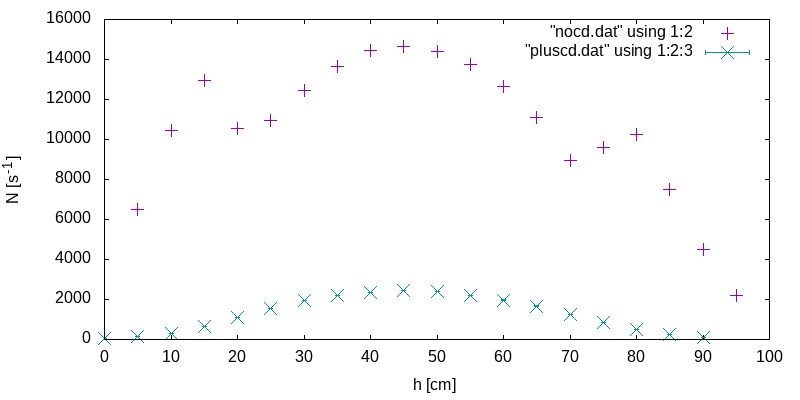
\includegraphics[width=0.4\textwidth]{both.png}
    \caption{Nějaký graf.}
    \label{fig:graf}
\end{figure}
\end{verbatim}

\begin{figure}[h]
    \centering
    \captionsetup{name=Graf}
    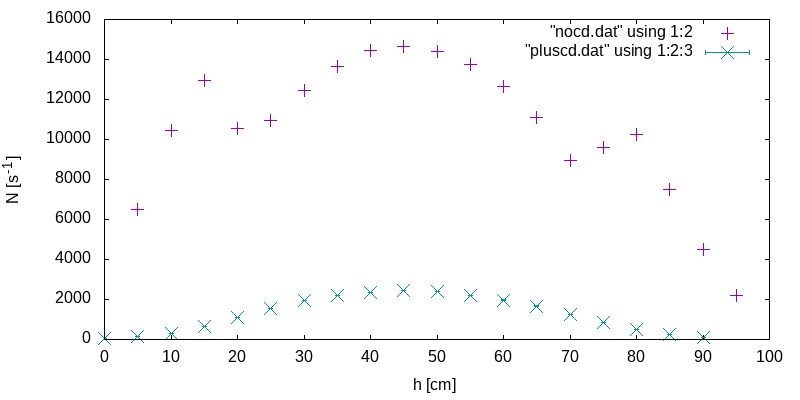
\includegraphics[width=0.4\textwidth]{both.png}
    \caption{Nějaký graf.}
    \label{fig:graf}
\end{figure}

Zkrácená verze pak je \verb|\graf{both.png}{Nejaky graf.}{fig:takygraf}|.
\graf{both.png}{Nejaky graf.}{fig:takygraf}

Je-li potřeba dát dva obrázky vedle sebe, lze použít \verb|minipage|.
\begin{verbatim}
    \begin{figure}[H]
        \centering
        \begin{minipage}{0.49\textwidth}
            \centering
            
\includegraphics[width=0.98\textwidth]{fjfi.pdf}
            \caption{Levý obrázek.}
            \label{fig:levy}
        \end{minipage}\hfill
        \begin{minipage}{0.49\textwidth}
            \centering
            
\includegraphics[width=0.98\textwidth]{symbol_cvut_konturova_verze_cb.pdf}
            \caption{Pravý obrázek.}
            \label{fig:pravy}
        \end{minipage}
    \end{figure}
\end{verbatim}

\begin{figure}[H]
    \centering
    \begin{minipage}{0.49\textwidth}
        \centering
        
\includegraphics[width=0.98\textwidth]{fjfi.pdf}
        \caption{Levý obrázek.}
        \label{fig:levy}
    \end{minipage}\hfill
    \begin{minipage}{0.49\textwidth}
        \centering
        
\includegraphics[width=0.98\textwidth]{symbol_cvut_konturova_verze_cb.pdf}
        \caption{Pravý obrázek.}
        \label{fig:pravy}
    \end{minipage}
\end{figure}

Podobně i zde existují zkrácené verze.
\begin{verbatim}
\dobr{fjfi.pdf}{Jeden obrazek. Zřejmě by bylo dobré udělat je stejně velké.
Proto v~obr.~\ref{fig:srovnany} nastavíme velikost pomocí nepovinneho
parametru.}{fig:prvni}{symbol_cvut_konturova_verze_cb.pdf}{Druhý obr.}{fig:druhy}
\end{verbatim}

\begin{verbatim}
\dgraf{both.png}{Jeden graf.}{fig:dalsi}{calibration.png}{Druhý graf.}{fig:ddalsi}
\end{verbatim}


\subsection{Kód}
Nejlepší metoda pro vkládání úryvků kódu je pomocí balíčku \verb|listing|.
Dobrý návod je na Overleafu \cite{overleaf_code_listing}.

\subsection{Citace}


\subsection{Odkazy}

\subsection{Indexy}

\subsection{Čeština}


\printbibliography[title={Literatura}]

\end{document}
